\documentclass[DM,authoryear,toc]{lsstdoc}
% lsstdoc documentation: https://lsst-texmf.lsst.io/lsstdoc.html
\input{meta}

% Package imports go here.

% Local commands go here.

%If you want glossaries
%\input{aglossary.tex}
%\makeglossaries

\title{Host Galaxy Association for DIAObjects}

% Optional subtitle
% \setDocSubtitle{A subtitle}

\author{%
M.~L.~Graham et al.
}

\setDocRef{DMTN-151}
\setDocUpstreamLocation{\url{https://github.com/lsst-dm/dmtn-151}}

\date{\vcsDate}

% Optional: name of the document's curator
% \setDocCurator{The Curator of this Document}

\setDocAbstract{%
This document describes the {\tt DIAObject} parameters that associate extragalactic transients with potential host galaxies, and which will be produced by the Alert Production pipeline and included in the alert packet. 
}

% Change history defined here.
% Order: oldest first.
% Fields: VERSION, DATE, DESCRIPTION, OWNER NAME.
% See LPM-51 for version number policy.
\setDocChangeRecord{%
  \addtohist{0}{2020-02-26}{Inception.}{Melissa Graham}
  \addtohist{1}{2020-05-11}{Pre-RFC.}{Melissa Graham}
  \addtohist{1.1}{2021-03-09}{Revision for DM-23683, RFC-695.}{Melissa Graham}
}


\begin{document}

% Create the title page.
\maketitle
% Frequently for a technote we do not want a title page  uncomment this to remove the title page and changelog.
% use \mkshorttitle to remove the extra pages

% % % % % % % % % % % % % % % % % % % % % % % % % %
\section{Introduction} \label{sec:intro}

The LSST Alert Production pipeline will will generate alert packets within $60$ seconds of image readout for all \textit{sources} detected during difference image analysis (DIA; {\tt DIASources}).
{\tt DIASources} are associated by sky coordinate into {\tt DIAObjects}, and a {\tt DIASource} at a sky coordinate with no previous detections from DIA becomes a new {\tt DIAObject}.

Individuals and brokers processing alerts will use the information in these packets to rapidly evaluate and prioritize {\tt DIAObjects} for follow-up with limited resources.
Thus the contents of the alert packet have been designed to contain a sufficient amount of LSST data about each {\tt DIAObject} to enable immediate analysis.

One important piece of information is the association of each {\tt DIAObject} with a static-sky {\tt Object} from the Data Release (DR) catalogs.
Brokers will use the {\tt Object} association to obtain data about the static-sky object from the DR catalogs, such as whether it might be galactic or extragalactic, at high- or low-redshift, nuclear or offset from a host, etc.
All of this information can help an alert stream user identify and prioritize their targets of interest, and delivering alerts \emph{with} the static-sky association already completed avoids the situation of multiple users cross-matching in real time.
This document describes the elements of the {\tt DIAObject} catalog that contain the {\tt Object} association parameters and describe how they will be calculated. 


\section{{\tt DIAObject}--{\tt Object} Association Parameters}\label{sec:params}

\subsection{Relevant to all transients and variables}\label{ssec:params_all}

With respect to associations between {\tt DIAObjects} and {\tt Objects}, the contents of the alert packet as defined in the Data Products Definitions Document (DPDD; \citeds{LSE-163}) includes the following:
\begin{itemize}
\item {\tt nearbyObj} ({\tt unit64[6]}), the {\it "closest {\tt Objects} (3 stars and 3 galaxies) in Data Release database"}
\item {\tt nearbyObjDist} ({\tt float[6]}), the {\it "distances to {\tt nearbyObj}"} in arcseconds
\item {\tt nearbyObjLnP} ({\tt float[6]}), the {\it "natural log of the probability that the observed {\tt DIAObject} is the same as the nearby {\tt Object}"}
\end{itemize}

For {\tt nearbyObjLnP}, a footnote states {\it "This quantity will be computed by marginalizing over the product of position and proper motion error ellipses of the {\tt Object} and {\tt DIAObject}, assuming an appropriate prior"}.
The definition of {\tt nearbyObjLnP} is only appropriate for static variable point sources (stars): for transients in host galaxies, the observed {\tt DIAObject} will never be ``the same as the nearby {\tt Object}".


\subsection{Relevant to extragalactic transients}\label{ssec:params_trans}

There are a wide variety of options to associate extragalactic transients with their host galaxies, as presented in Section \ref{sec:options}. 
Typically, radial distances in arcseconds are not used in favor of a \emph{separation distance} which accounts for the galaxies' spatial luminosity profiles \citep[e.g.,][]{2006ApJ...648..868S}.

To associate {\tt DIAObjects} with DR {\tt Objects}, a separation distance calculated from the galaxies' second moments (Section \ref{ssec:options_mom}) will be used to generate {\tt DIAObject} elements:
\begin{itemize}
\item {\tt potentialHost} (unit64[3]), the {\tt objectId} for the three {\tt Object} catalog extended sources with the lowest separation distances
\item {\tt potentialHostSeparation} (float[3]), the separation distances for each {\tt potentialHost}
\end{itemize}

\subsubsection{A manageable computational load.}\label{sssec:params_trans_comp}
All of the parameters that are required in order to calculate the separation distances, as described in Appendix \ref{sec:appA}, will already exist in the {\tt DIAObject} and {\tt Object} tables.
Separation distances need not be calculated for \textit{all} {\tt Objects}; a suitable limit would be to calculate separation distances for {\tt Objects} within $\sim$90\arcsec.
A galaxy with a diameter of 25 kpc (i.e., like the Milky Way) has an angular diameter of $\\sim$30\arcsec at a distance of 200 Mpc ($z\sim0.045$).
Thus, considering all galaxies within $\sim$90\arcsec could associate a low-redshift transient at $\sim$3 effective radii ($R_e$) from its host galaxy.
There would be $\sim$400 background galaxies within this $\sim$90\arcsec radius (scaled from the $\sim$4 billion galaxies expected in the full $\sim$18000 deg$^2$ of the wide-fast-deep main survey), 
This means that just $\sim$400 separation distances would need to be calculated for each {\tt DIAObject} in order to fill the above table elements. 

\subsubsection{Failure for low-redshift transients.}\label{sssec:params_trans_fail}
In Appendix \ref{sec:appB} we show that up to 1\% of such low-redshift transients would randomly fall within $3R_e$ of three background interloper galaxies, and the true host would not be included in {\tt potentialHost}.
This issue is exacerbated for low-redshift transients further in the outskirts of their large host galaxies, or transients in the Local Volume -- both of which have a very high scientific value for follow-up programs.
Furthermore, large, extended, low-redshift galaxies are likely to be significantly fragmented in the DR {\tt Objects} catalog, with plenty of ``child" {\tt Objects} that would complicate host association.
These issues with low-redshift host association \textit{could} be mitigated by reporting a larger number of nearby potential hosts, or by dedicating significant (and currently out of scope) effort to building a low-redshift DR {\tt Object} catalog, but Section \ref{ssec:params_lowz} presents a more straightforward solution to low-redshift host association.


\subsection{Relevant to low-redshift extragalactic transients}\label{ssec:params_lowz}

An established catalog of low-redshift galaxies (e.g., from the NGC/IC list of $\lesssim$14000 Revised New General Catalogue and Index Catalogue; TBD) will be adopted, and all new {\tt DIAObjects} will be cross-matched to it during Alert Production in order to report the name and the radial sky separation of the nearest catalog galaxy:
\begin{itemize}
\item {\tt potentialLowzHost} (str[1]), the catalog name of the nearest ?low-z? potential host
\item {\tt potentialLowzHostSeparation} (float[1]), the distance to {\tt potentialLowzHost} [arcsec]
\end{itemize}

If the community provides a catalog of names and coordinates that they would prefer to be used, it will be adopted. 
If that catalog includes more information about the galaxy, then the value of {\tt potentialLowzHostSeparation} could be more sophisticated than the radial distance in arcseconds. 
For example, if distances are included then the offset in kpc could be provided; if sizes are included the number of effective radii could be reported; or if the second moments are included then the separation could be the same as used for {\tt potentialHostSeparation}. 




\section{A Discussion of Options for Host Galaxy Association}\label{sec:options}

Statistically, the most likely host for a given transient is the galaxy which contributes the most optical flux at the transient's location.
This is usually estimated by first calculating a \emph{separation distance} from the nearby galaxies to the transient which is expressed in terms of the galaxy's spatial luminosity profile, and then assuming the galaxy with the lowest separation distance is the host.
The following are several options for estimating which nearby galaxy is the most likely host of an extragalactic transient.

\subsection{Effective Radius}\label{ssec:options_Re}

For the separation distance, use the radial distance from the core of the galaxy to the location of the transient, divided by the effective radius of the galaxy.
The DR {\tt Objects} table is already planned to contain suitable effective radii such as the parameter {\tt kronRad90} \citedsp{LSE-163}.
This option for the separation distance would not require any additional processing aside from dividing the radial distance from transient to {\tt Object} by the effective radius of the {\tt Object}.
Although this kind of separation distance would account for the relative sizes of the potential host galaxies, it does not account for their position angles, and so would not be as accurate for assessing potential high-inclination host galaxies.

\subsection{Second Moments}\label{ssec:options_mom}

This method calculates a separation distance based on the two-dimensional luminosity profile of the nearby galaxies.
For example, \citet{2006ApJ...648..868S} describe the method applied to the Supernova Legacy Survey (SNLS), using a separation distance of $R^2 = C_{xx} x_r^2 + C_{yy} y_r^2 + C_{xy} x_r y_r$, where $C_{xx}$, $C_{yy}$, and $C_{xy}$ are ellipse parameters derived from the second moments of the galaxy luminosity profile and $x_r$,$y_r$ are the on-sky distances between the centroids of the transient and the galaxy.
The DR {\tt Objects} table is already planned to contain the second moments of the galaxy luminosity profiles ({\tt Ixx}, {\tt Iyy}, and {\tt Ixy}; \citeds{LSE-163}).
A step-by-step description of how this separation distance can be calculated from planned {\tt DIAObject} and {\tt Object} table elements is provided in Section \ref{sec:appA}.

Multiple recent surveys have used this method (or similar) to associate transients with their host galaxies, such as \citet{2018PASP..130f4002S} for SDSS supernovae, and \citet{2016AJ....152..154G} who use real and simulated data to evaluate the optimal method for host association.
This option for the separation distance requires more computational steps than effective radius, but accounts for both the relative sizes and position angles of the potential host galaxies. 

\subsection{Hierarchical Associations}

Instead of associating a {\tt DIAObject} with the three extended {\tt Objects} with the lowest separation distance, another option is to associate the {\tt DIAObject} with the  nearest {\tt Object} at three different size scales.
For example, the nearest $R_e<10"$ neighbor within $d<100"$ (high-$z$ and small galaxies), the nearest $R_e<100"$ neighbor within $d<1000"$ (large low-$z$ galaxies), and the nearest $R_e<1000"$ neighbor within $d<10000"$ (very large nearby galaxies).
In this option, the ``nearest neighbor" in a given scale bin could be determined using a separation distance calculated from, e.g., the second moments (Section \ref{ssec:options_mom}).

However, this option does not avoid the issue of contamination by background galaxies as discussed in Appendix \ref{sec:appB}.
To mitigate background interlopers, the nearest \emph{three} extended sources for \textit{each} size scale should be included.
This is less necessary for the largest size scale, but it would assist with identifying transients in galaxy groups and clusters, especially the rare transients with large offsets which might belong to intracluster stellar populations.

This option of hierarchical associations would require three times as much storage space in the {\tt DIAObject} catalog.
Although this option might reduce the number of {\tt Objects} for which a separation distance must be calculated for each {\tt DIAObject}, as described in Section \ref{ssec:params_trans} this number is only $\sim$400 (i.e., not overwhelmingly large). 

Ultimately, the largest size scale would face the same issues for low-redshift galaxies as described in Section \ref{sssec:params_trans_fail}. 
This method of hierarchical associations is thus not adopted for the Alert Production pipeline, as the combination of the methods described in Section \ref{ssec:params_trans} and \ref{ssec:params_lowz} will, together, adequately cover the science needs.

\subsection{2D Algorithms and Footprints}

Aside from adopting a separation distance, there are more complicated methods for identifying the most likely host for a given transient.
For example, the nearby galaxy with the smallest fraction of light interior to an isophot through the transient's location, where the isophot shape is given more degrees of freedom and not constrained to concentric ellipticals as in the second moment method above.
Another example is to use an algorithm that provides deblended footprints for nearby extended objects, and that can estimate the fraction of light in given pixel that should be attributed to each (e.g., as the SCARLET deblender can do, \cite{2018A&C....24..129M}).
The most likely host galaxy would be the one which contributes the most flux at the pixel location of a transient.
While all DR {\tt Objects} will be associated with a footprint (a region of connected pixels), the footprint information will not be stored in the {\tt Object} table.
The use of footprints in identifying potential host galaxies would require more computational resources during Alert Production, but would probably return a more accurate host association for only a very small fraction of {\tt DIAObjects}. 

Methods based on 2D algorithms or footprints are thus not adopted for the Alert Production pipeline, but might be applied by science users in their analysis of the Data Release data products. 

\subsection{Galaxy/Transient Types}

The association of transients with their host galaxy can be more accurate if their properties are also considered.
For example, the potential host galaxy's redshift can be used to calculate separation distances in physical units, or to estimate the absolute brightness of the transient and consider whether it is physically plausible.
Priors based on the established correlations between transient types and host galaxy morphology or color can also be used to refine a probabilistic host association, such as how core collapse supernovae are almost always associated with star formation (except for a few notable cases, e.g., \citealt{2012ApJ...753...68G,2019ApJ...887..127I}).
A demonstration that these correlations between host and transient types are so robust that the host type can be used to provide a statistical classification of the transient type was presented by \citet{2013ApJ...778..167F}.

However, making science-informed associations between transients and galaxies based on any kind of derived properties is beyond the scope of Alert Production, and is best left to the users on a case-by-case basis. 
Thus, properties of the transients and/or the nearby galaxies (beyond their coordinates and luminosity profile) should not be used during the association of {\tt DIAObjects} and {\tt Objects}.

For a very thorough assessment of an optimized, science-driven system for associating supernovae and their host galaxies -- including the role and performance of machine learning methods -- we direct the reader to \citet{2016AJ....152..154G}.

\subsection{Identifying Hostless Transients}

For some scientific analyses, transients which are $>$3-5 effective radii away from the nearest galaxy, or for which $>99\%$ of the potential host's luminosity is within the radial distance between transient and host center, are considered ``hostless" (e.g., \citealt{2011ApJ...729..142S}).
Such a cutoff has been appropriate for past samples of $\sim$hundreds of transients, but will not be appropriate for the LSST sample size.
Furthermore, the decision of whether and how to consider a transient ``hostless" is best left as a scientific decision for the end-user.
Thus, no such cut should be applied during the association of {\tt DIAObjects} and {\tt Objects}, and the most likely hosts should still be reported, even if the probability is low.


\clearpage
\section{Appendix A: Separation Distance from Second Moments}\label{sec:appA}

From the LSST catalogs the following {\tt Object} table elements are used to define the parameters needed to calculate the separation distance \citedsp{LSE-163}:

\begin{center}
\begin{tabular}{ccll}
\hline
Parameter & Unit & Table Element & Description \\
\hline
$x_{\rm trans},y_{\rm trans}$ & $\rm degrees$ & {\tt DIAObject} {\tt radec} & transient centroid  \\
$x_{\rm gal},y_{\rm gal}$       & $\rm degrees$ & {\tt Object} {\tt radec}       & galaxy centroid      \\
$\overline{x^2}$,$\overline{y^2}$,$\overline{xy}$ & $\rm arcsec^2$  & {\tt Object} {\tt Ixx}, {\tt Iyy}, {\tt Ixy} & galaxy second moments \\
\hline
\end{tabular}
\end{center}

There might be an issue with using the {\tt Object} catalog second moments: the {\tt Ixx}, {\tt Iyy}, and {\tt Ixy} are defined with with respect to the local tract/patch and not sky coordinates (Jira DM-19519).
Although the local tangent projection will probably work fine for this application of the second moments, this should be verified at the time of implementation.

As described in Section 10 of E. Bertin's Source Extractor manual\footnote{Version 2.3: \url{https://www.astromatic.net/pubsvn/software/sextractor/trunk/doc/sextractor.pdf}} (and presumably many other places), the unitless ellipse parameters $C_{xx},C_{yy},C_{xy}$ can be calculated from the second moments via:

\begin{equation}
C_{xx} = \frac{\overline{y^2}}{\sqrt{ \left( \frac{\overline{x^2}-\overline{y^2}}{2} \right)^2 + \overline{xy}^2}}
\end{equation}

\begin{equation}
C_{yy} = \frac{\overline{x^2}}{\sqrt{ \left( \frac{\overline{x^2}-\overline{y^2}}{2} \right)^2 + \overline{xy}^2}}
\end{equation}

\begin{equation}
C_{xy} = -2 \frac{\overline{xy}}{\sqrt{ \left( \frac{\overline{x^2}-\overline{y^2}}{2} \right)^2 + \overline{xy}^2}}
\end{equation}

The sky distances between the transient and galaxy centroids are calculated as follows, and include the $\cos(\delta)$ factor and a conversion from units of degrees to arcseconds:

\begin{equation}
x_r = 3600(x_{\rm SN} - x_{\rm gal})
\end{equation}

\begin{equation}
y_r = 3600(y_{\rm SN} - y_{\rm gal})\cos{y_{\rm gal}}
\end{equation}

Finally, the separation distance $R$ in arcseconds is given by:

\begin{equation}
R^2 = C_{xx} x_r^2 + C_{yy} y_r^2 + C_{xy} x_r y_r.
\end{equation}
 %\label{sec:appA}

\clearpage
\section{Appendix B: Overcoming Background Galaxy Contamination}\label{sec:appB}

In this appendix, the probability of failed host galaxy associations for nearby transients with large host offsets due to interloping background galaxies is quantified, and used to evaluate the minimum number of potential hosts that should be stored in a {\tt DIAObect} record. 
For simplicity, this appendix uses the effective radius as the separation distance (Section \ref{ssec:options_Re}).

The 10-year {\tt Object} catalogs will include $\sim$4 billion galaxies with $i<25$ mag across the $\sim$20000 $\rm deg^2$ main survey area, known as the ``gold" sample, especially in the context of weak lensing studies \citedsp{LPM-17}.
However, the 10-year coadded depths will detect galaxies down to 5$\sigma$ limiting magnitudes of 26.1, 27.4, 27.5, 26.8, 26.1, and 24.9 mag in filters {\it ugrizy}; this is $\sim$3 times as many as in the ``gold" sample, or $\sim$10 billion galaxies.
This high density of background galaxies complicates the process for associating large nearby host galaxies with their transients, especially the rare transients in their outskirts.

Consider a transient at $3R_e$ from the center of a nearby galaxy with $z=0.01$ and an effective radius of $R_e = 10$ kpc ($\sim$50 arcsec).
In order for this transient to be associated with it's true host, the separation distance for all {\tt Objects} within a radius of at least $3R_e$, and thus an area of at least $A_{3R_e} = \pi (3R_e)^2 = 0.0052$ $\rm deg^2$, would need to be considered.
Based on the final 10-year number of detected galaxies (10 billion) and the total survey area (20000 deg$^2$), that is $\sim (10^10 / 20000) \times 0.0052 \approx 2600$ galaxies.
Furthermore, the true host galaxy must have a lower separation distance than the $N$ nearest background galaxies, where $N$ is the number of potential hosts that will be listed in the {\tt DIAObject} parameters {\tt potentialHost} and {\tt potentialHostSeparation}.

\begin{figure}[h]
\begin{center}
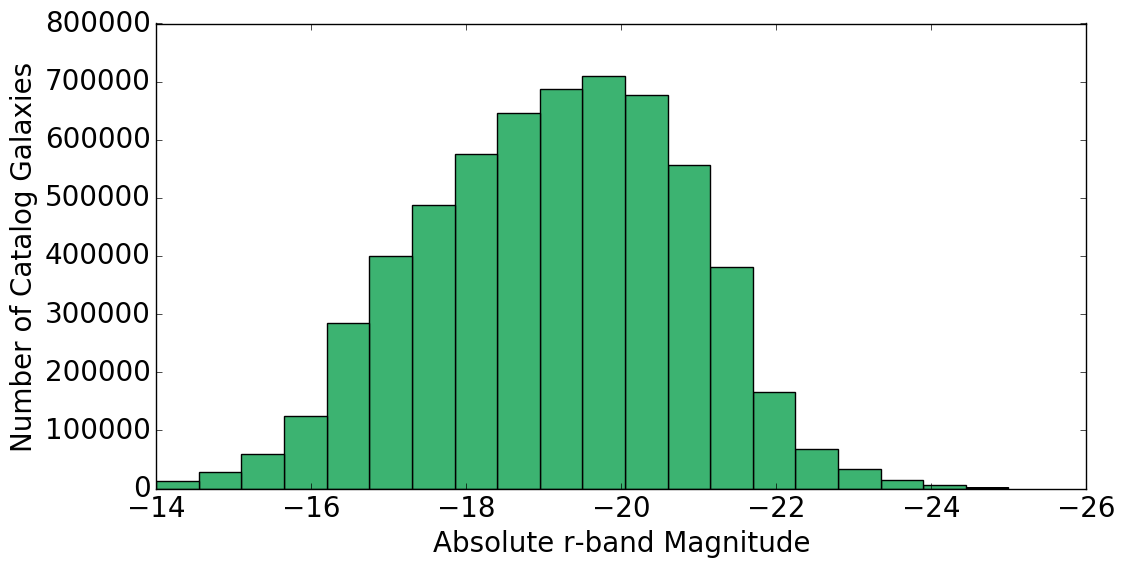
\includegraphics[width=8cm]{hg_Mr_dist.png}
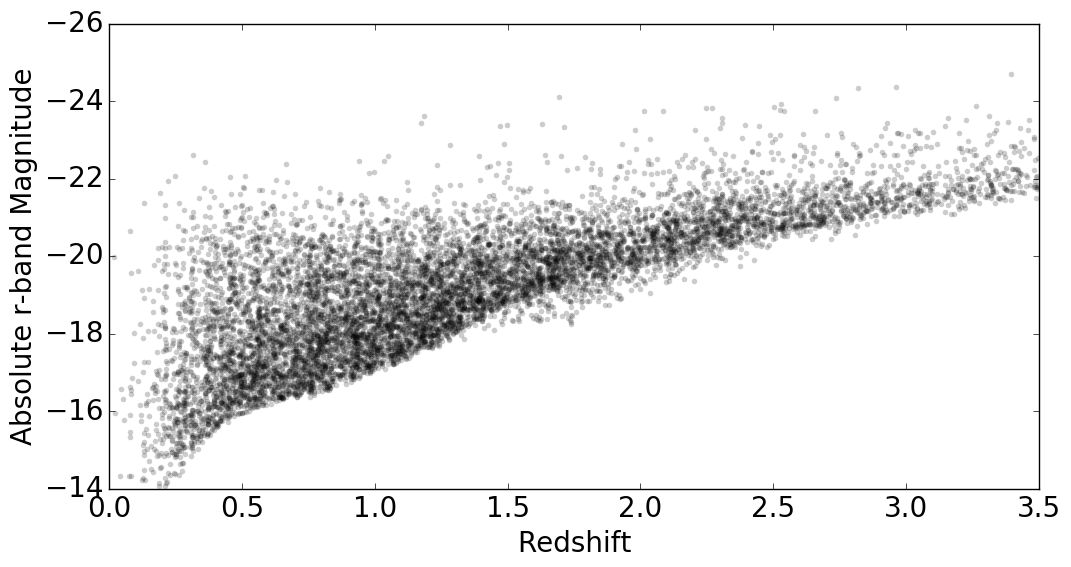
\includegraphics[width=8cm]{hg_Mr_vs_z.png}
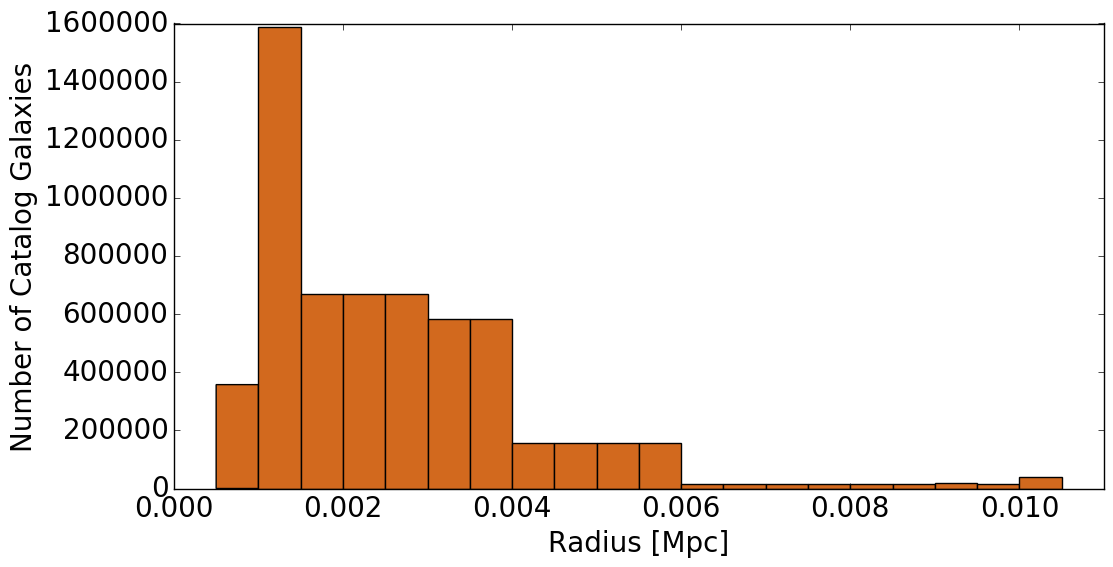
\includegraphics[width=8cm]{hg_rad_dist.png}
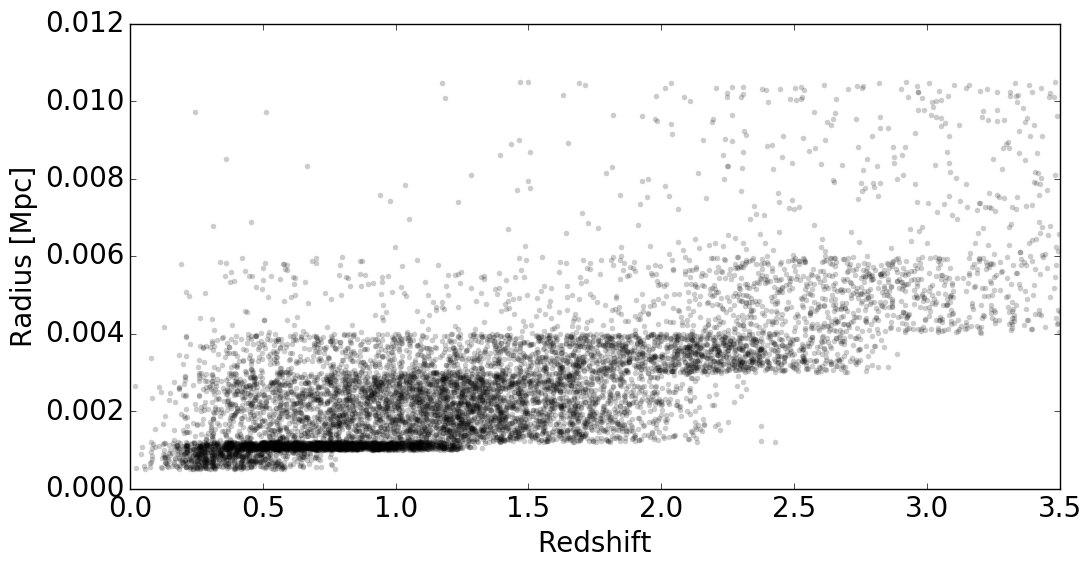
\includegraphics[width=8cm]{hg_rad_vs_z.png}
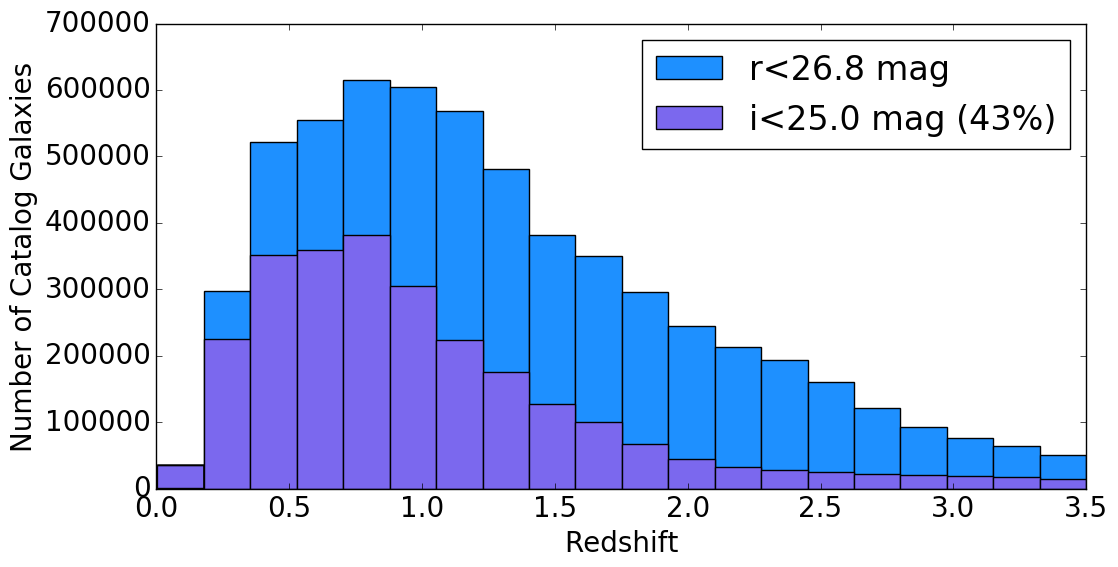
\includegraphics[width=8cm]{hg_z_dist.png}
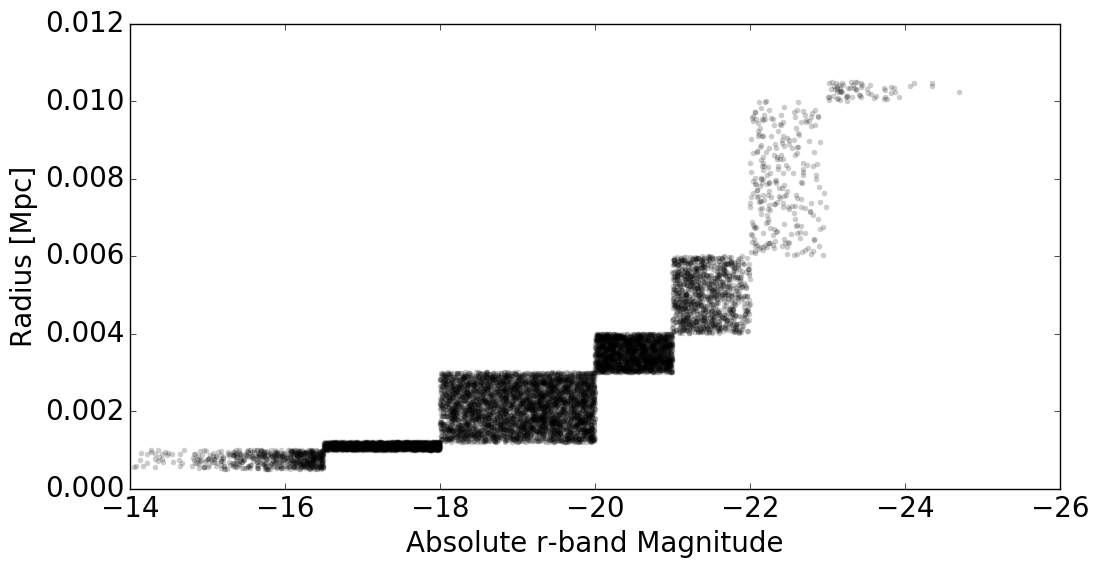
\includegraphics[width=8cm]{hg_rad_vs_Mr.png}
\caption{{\it Left:} Histograms of the synthesized absolute $r$-band intrinsic magnitude (top) and radius (middle) for catalog galaxies, and the simulated galaxy redshifts (bottom). {\it Right:} Correlation with redshift of the synthesized intrinsic magnitude (top) and radius (middle), and the approximate relation between radius and intrinsic magnitude (bottom).  \label{fig:simcat}}
\end{center}
\end{figure}

To investigate the probability of host-association failure for nearby transients, we simulate a mock catalog of randomly distributed random background interloper galaxies.
It is based on the same LSST-like mock galaxy catalog used by \citet{2018AJ....155....1G} for studies of photometric redshifts.
For this experiment the catalog is limited to galaxies with at least a 5$\sigma$ detection in the {\it griz} bands at the projected 10-year depths listed above.
The catalog contains redshifts and apparent {\it ugrizy} magnitudes, which are used to approximate intrinsic absolute $r$-band magnitudes (without $K$-correction, simply using a distance modulus based on redshift and $M_r=m_r-\mu$).
The absolute magnitudes are used to synthesize approximate galaxy radii based on the relationship between absolute magnitude and radius for late-type galaxies defined in Figure 3 of \citet{2003MNRAS.343..978S}.
These synthesized radii are over-estimates because late-types are generally larger than early-types, and because this magnitude-radius relation was defined for SDSS galaxies at lower redshifts than the LSST high-$z$ galaxies it is being applied to.
This is a deliberate choice to overestimate, because it will result in upper limits on the rate of interlopers, which will allow for conservative estimates about the effect of background interlopers.
The characteristics of this crude galaxy catalog are illustrated in Figure \ref{fig:simcat}.

Consider again the large nearby galaxy with $R_e=10$ kpc at a redshift of $z=0.01$, for which the sky area within $3R_e$ is $A(3R_e)=0.0052$ $\rm deg^2$ and contains $\sim$2600 background galaxies.
From the simulated catalog described above, 100 sets of background galaxies are randomly selected.
For each set, the fraction of the nearby galaxy's area which is covered by the area of interloping background galaxies is calculated: $f_A = \sum{A(3R_{e,{\rm bkg}})} / 0.0052$.
This fraction is equivalent to the probability that a transient at $3R_e$ from this large nearby host will be within $3R_{e,{\rm bkg}}$ (i.e., will be closer to) a background interloper.
The probability that this transient is closer to $N$ interlopers than to its true host is $P_{\rm fail} = (f_A)^N$.
This is the probability of a failed host association, where ``failed" means that the {\tt DIAObject} record of the $N$ galaxies with the lowest separation distances does not include the true host.
For this large nearby galaxy, average values of $f_A$ and $P_{\rm fail}$ from the 100 simulated background sets are $f_A = 0.181\pm0.008$ and $P_{\rm fail} (N=3) = 0.006\pm0.0008$

Since this probability of failure is based on the sky density of background galaxies, it is independent of the radius and redshift of the nearby galaxy. 
However, it does depend on the factor applied to effective radius (i.e., the offset of transient considered) and $N$, the number of potential hosts recorded in the {\tt DIAObject} catalog.
Figure \ref{fig:pfail} shows the probability of failure as a function of $R_e$ and $N$.
\textbf{These are upper limits on the probability of failure} because they are derived from upper-estimates of galaxy radii and the sky density of the final 10-year LSST galaxy catalog, as described above. 

To assist in the interpretation of Figure \ref{fig:pfail}, the following describes several conclusions drawn from points in this plot:
\begin{itemize}
\item Transients with low host offsets, $1R_e$, are closer to (within $1R_{e,{\rm bkg}}$ of) one background interloper $\sim2\%$ of the time (purple point at $1R_e$). (However, given the high surface brightness of nearby galaxies, such a background galaxy might not be detected.)
\item Transients with high host offsets, $5R_e$, are closer to (within $5R_{e,{\rm bkg}}$ of) one background interloper $\sim50\%$ of the time (purple point at $5R_e$), and closer to six background interlopers $>1\%$ of the time (magenta point at $5R_e$).
\item In order to achieve a $1\%$ probability of failure for transients offset by $3R_e$ from large nearby galaxies, the {\tt DIAObject} catalog record should include the $N=3$ galaxies with the lowest separation distances (green point at $3R_e$).
\end{itemize} 

All of the above experiment can be summarized in two main recommendations aimed at reducing the probability of failure in associating nearby, large-offset transients with their true hosts:
\begin{enumerate}
\item The separation distances for all galaxies within at least $4R_e \approx 200$ arcsec should be calculated and considered.
\item The 3 galaxies with the lowest separation distances should be included in the {\tt DIAObject} catalog record.
\end{enumerate}
Adopting these recommendations would cause up to $1\%$ of the transients at $3R_e$ from large nearby galaxies to experience a failed host association, where the true host is not listed in the {\tt DIAObject} record.
Since $3R_e$ encompasses $\sim99\%$ of a galaxy's light, and most transient types are distributed proportional to the light, \textbf{the upper limit on the host association failure rate} for nearby transients should be $\sim0.01\%$.

\begin{figure}[h]
\begin{center}
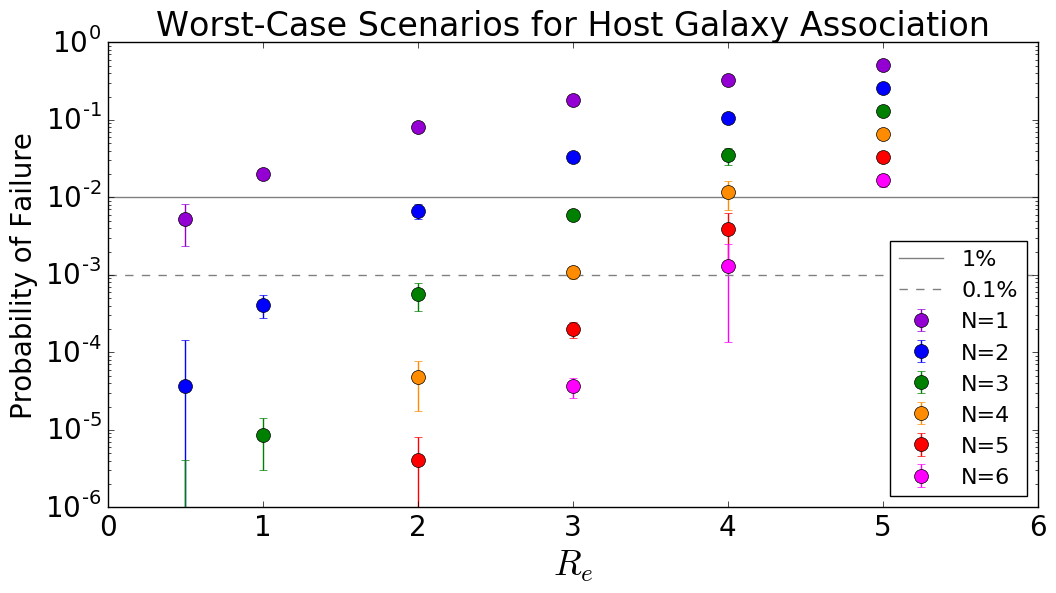
\includegraphics[width=12cm]{hg_P_vs_Re.png}
\caption{The probability that a transient will fail to be associated with a large ($R_e=10$ kpc) nearby host galaxy due to background interlopers, as a function of the transient's offset in effective radii from galaxies in the vicinity (including the true host), where ``failure" means the true host's separation distance is not in the top $N$ nearest galaxies. \textbf{This is a ``worst case scenario" because it applies to an very large nearby galaxy, and all background galaxy radii estimates are upper limits} (as described in the text). Error bars show the standard deviation from the 100 randomly-generated sets of background galaxies. \label{fig:pfail}}
\end{center}
\end{figure}
 %\label{sec:appB}


\clearpage

\appendix
% Include all the relevant bib files.
% https://lsst-texmf.lsst.io/lsstdoc.html#bibliographies
\section{References} \label{sec:bib}
\bibliography{local,lsst,lsst-dm,refs_ads,refs,books,mlg}

% Make sure lsst-texmf/bin/generateAcronyms.py is in your path
\section{Acronyms} \label{sec:acronyms}
\input{acronyms.tex}
% If you want glossary uncomment below -- comment out the two lines above
%\printglossaries

\end{document}
